\chapter{Design}

\section{Denavit-Hartenberg}

In order to enable the UR5 on the flexible workstation to locate itself and its surroundings within a space, the DH (Denavit-Hartenberg) method is used.\\ 
The DH method is a method which can be used to compute every joint/axis into parameters of the coordinate systems.\\
These descriptions of the system can be used to translate every point and every movement of the robotic manipulator, with the help of forward kinematic.\\
Initially the start is to locate all of the coordinate systems, as seen in \ref{table:DH-table}.\\ 


\begin{itemize}
    \item ${a_{i-1}}$= The distance from ${Z_{i-1}}$ to ${Z_{i}}$ measured along ${X_{i-1}}$
    \item ${\alpha_{i-1}}$ = The angel between ${Z_{i-1}}$ to ${Z_{i}}$ measured about ${X_{i-1}}$
    \item ${d_{i}}$ = The distance from ${X_{i-1}}$ to ${X_{i}}$ measured along ${Z_{i}}$
    \item ${\theta_{i-1}}$ = The angel between ${X_{i-1}}$ to ${X_{i}}$ measured about ${Z_{i}}$
\end{itemize}


\newpage

Then the angles and the distance from each coordinate system is computed and set in to a table as seen in \ref{fig:DH-Table}.

\begin{figure}[h]
    \centering
    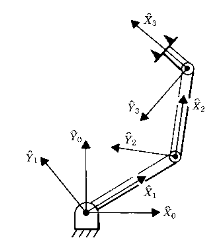
\includegraphics[scale=1]{Design/DHmani.PNG}
    \caption{Manipulator for describing DH-parameters \cite{DH}} 
    \label{fig:DH-Table} 
\end{figure}

\begin{table}[h!]
\centering
\begin{tabular}{||c c c c c||} 
 \hline
 i & \alpha_{i-1} & a_{i-1} & d_{i} & \theta_{i} \\ [0.5ex] 
 \hline\hline
 1 & 0 & 0  & 0     & \theta_{1} \\ 
 2 & 0 & l_{1} & 0 & \theta_{2} \\
 3 & 0 & l_{2} & 0 & \theta_{3} \\[1ex]
 \hline
\end{tabular}
\caption{DH-Table}
\label{table:DH-table}
\end{table}

As seen in \ref{fig:DH-Table},the coordinate systems is used to trace every step of each axis.\\
Starting from left to right at the top of the table, the alpha-1 is used to compute the difference between the angle between Zi and Zi-1, which is 0, due to the fact that they keep the same angle from Zi to zi-1.\\
It can also be seen from the table that the distance between Zi and Zi-1 is Length2, since they are parallel to each other.\\ 
The distance between Xi-1 and Xi is 0 since they cross each other on the perpendicular line, which means that in that point the new coordinate system should be placed.\\
\newpage
\subsection{DH parameters for UR 5}


\begin{table}[h!]
\centering
\begin{tabular}{||c c c c c||} 
 \hline
 i & \alpha_{i-1} & a_{i-1} & d_{i} & \theta_{i} \\ [0.5ex] 
 \hline 
 \hline
 1 & 0 & 0 & 89.2 & \theta_{1} \\ 
 2 & 90 & 0 & 0 & \theta_{2} \\
 3 & 0 & 425 & 0 & \theta_{3} \\
 4 & 0 & 392 & 109.3 & \theta_{4} \\
 5 & 90 & 0 & 94.75 & \theta_{5} \\ 
 6 & -90 & 0 & 82.5 & \theta_{6} \\[1ex] 
 \hline
\end{tabular}
\caption{DH-parameters for the UR5, using \cite{DHPar} as measurement}
\label{table:1}
\end{table}

\section{Forward Kinematics}
Through the use of forward kinematics, it is possible to calculate the position of the end-effector, by using the joint angles, the most used method is Denavit-Hartenberg's computation method for forward kinematics, which is described in "John J. Craig - Introduction to robotics"\cite{JohnC}.\\
The computation sequence starts from the base of the robot manipulator, and goes through all the chains of links, aswell as joints, and ends at the position of the end-effector.\\
A six step method is used to acquire the joints coordinate frames.\\
\begin{itemize}
    \item Step 1: Identify the joint axis's, and draw a line for each of the identified joint axis's, as shown on figure \ref{fig:FK1} with the red lines.
    \item Step 2: A common orthogonal is identified. If the axis's do not intersect with each other, then the shortest distance between them, has to be found, as indicated by the green lines on figure \ref{fig:FK1}.
    \item Step 3: The Zi axis, should be assigned to be in the same direction as the axis's of the joints. As indicated on figure \ref{fig:FK2}.
    \item Step 4: The Xi axis of the joint frame, has to be assigned the same as the common orthogonal of the two frames. If the two frames intersect with each other, the Xi axis is assigned as to be the normal to the plane, containing those two axes. On figure \ref{fig:FK2} Xi has been assigned as the orthogonal, because there are no intersecting joint frames in the example.
    \item Step 5: The Yi axis can be completed by using a standard coordinate system. This step is optional, for the reason that the Yi axis is not really being used. 
    \item Step 6: Assign as many link parameters as possible to be the value of zero, to ease the calculations.
\end{itemize}

\begin{figure}[h]
    \centering
    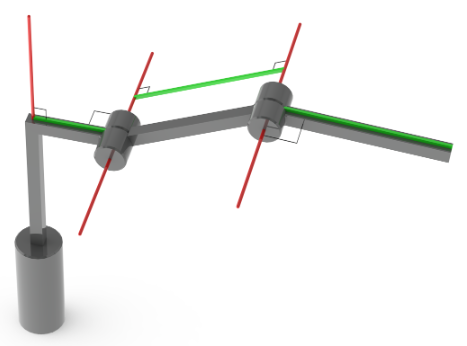
\includegraphics[width=9cm]{Design/FK1.PNG}
    \caption{Figure of step 1 and 2, the red lines are the join axes, and green is the orthogonal between the axis's\cite{KinePics}.}
    \label{fig:FK1}
\end{figure}

\begin{figure}[h]
    \centering
    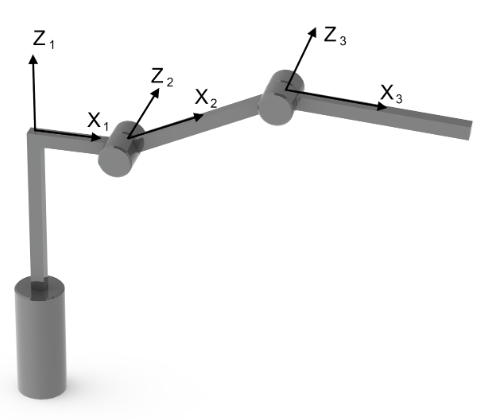
\includegraphics[width=9cm]{Design/FK2.PNG}
    \caption{Step 3,where the Z and X axis is assigned to form a plane\cite{KinePics}.}
    \label{fig:FK2}
\end{figure}


\newpage
\section{Inverse Kinematics}
Inverse kinematics is used to compute the joint angles from a given position and orientation of an object\cite{JohnC}. The inverse kinematic can by setup from two aspects, one is that geometric way and the other is an algebraic solution, the one the team is using is the algebraic solution where the inverse kinematics is setup in maple, a math computer program, where it makes it possible to be used later in computing the trajectory of the manipulator.\\
\section{Conclusion}

Describing a robot with forward kinematics and Denavit-Hartenberg parameters is used to locate the different joints and the tool in 3D-space, so the robot can be manipulated and used for various tasks.\\
Looking at Denavit-Hartenberg, the advantage of this method is to simplify the different axis in a matrix, so the operator and the robot can identify where the different coordinate systems is located.\\
Forward kinematics is the starting point of selecting the DH-parameters, when we know the point Z1-1 and Z1 we can then locate every axis in the desired robot. Hereby conclude to DH-parameters and include them into Matlab and visualize the robot and locate the robot so the tasks can be performed.\\

\chapter{Ideal Work-cell}\label{IdealWorkCell}

-> Billede af workcell med mål og reach.\\

When looking at \ref{}, a reachable and systematic work-cell is presented. But the important thing of a work-cell is its flow.\\
Here is some sections about what is needed of the ideal work-cell.

\section{Dexterous workspace}

The workspace which a manipulator works within can be described as a radius which the point of the end-effector can reach.\\
The Dexterous workspace is a more intelligent way of the robot to decide which points in arbitrary orientation, can be reached \cite{Dexterous}.\\
The reason that the dexterous workspace is considered a solution to the work-cell, is that the kinematic restrains can be included, so that the trajectories of the manipulator wont freeze or go in lockdown.\\


\section{Safety}

To keep the production safe and manageable, some of the safety devices is chosen:

\begin{itemize}
    \item Light Curtain
    \item Lidar
\end{itemize}

The light curtain provides a signal when the curtain is broken, see \ref{SafetyDevices}.\\
This will be used to send a signal to the UR5 to either stop or slow down the production, so a person safely can enter the cell, without getting serious damages.\\

The Lidar is commonly used in production, see \ref{SafetyDevices}.
This threshold can be used to measure when a person enters a hazardous distance towards the UR5.\\
All of the above is a must since the UR5 is carrying a metal rotor with sharp edges, so the person wont be gauged.\\

\subsection{Safety Requirements}

The most important solution for the safety of the work-cell, is the ISO 10218-2:2011, see \ref{ISO2}.\\
When installing a new robot for a production line, some standards is required. These standards of the ISO can present which of the areas needed to be looked at.\\

\section{Placement Sensors}

To ensure the work-flow some intelligent placement sensors must be implemented. Some of the possible solutions is chosen:\\

\begin{itemize}
    \item Lidar
    \item Photocell sensors
    \item Depth sensing camera
\end{itemize}

The Lidar is a sensor that gives a concentrated 2D view, and can be used for the robot to tell the different object apart, and give an overview of the work-cell, see \ref{ref:PlacementS}.\\
These signals can be used for the cobot to get a better work-flow and also determine objects from each other.\\

The photocell sensors can be used for a quicker work-flow, since it will detect the rotors when they are in the correct place to be picked up, see \ref{ref:PlacementS}.\\

Depth sensing cameras can determine the distance from end-effector to the desired object, see \ref{ref:PlacementS}. This can be used to derive the distance from the certain machine where the rotor has to be placed.\\
When located the trajectory of the placement of the rotor can be simplified.

\chapter{Ideal Robot}\label{IdealRobot}